\chapter{Identità digitali}
L'autenticazione con password rappresenta spesso anche un rischio per la privacy dell'utente: molti fornitori di servizi mantengono altre info personali richieste all'utente per il rilascio di user e password (es: nome, cognome, mail, indirizzo fisico, ...). Se il fornitore del servizio è soggetto ad un databreach, l'utente rischia la diffusione dei suoi dati. Inoltre il fornitore, se soggetto a databreach, è costretto a pagare una multa salata (GDPR) in quanto non ha protetto adeguatamente i dati personali degli utenti.

Quindi i sistemi di autenticazione con password rappresentano problemi sia per l'utente che per il fornitore. 

Tutti questi problemi possono essere risolti dai sistemi di gestione dell'identità digitale. In questi sistemi il processo di autenticazione viene delegato dai fornitori dei servizi al sistema di identità digitale stesso, che si occuperà di verificare l'identità dell'utente nel momento in cui vuole accedere al servizio online. Le credenziali e le eventuali info associate vengono mantenute dal sistema di identità digitale. 
Questo solleva il service provider dall'implementare il sistema di autenticazione e da eventuali sanzioni derivanti da attacchi che rivelano le info personali degli utenti. 
Per gli utenti, previene che questi debbano mantenere credenziali potenzialmente diverse per ciascuno dei servizi online a cui vogliono accedere. L'utente deve infatti mantenere un solo set di credenziali, rilasciato da servizio di identità digitale, che utilizzerà per accedere ai vari servizi. 

\section{Identità digitale}
Un'identità digitale è un insieme di attributi che identificano l'utente, come:
\begin{itemize}
    \item Nome e cognome;
    \item User e password;
    \item Numero della carta di identità/passaporto;
    \item Indirizzo;
    \item Ruolo all'interno dell'organizzazione;
    \item Email;
    \item ...;
\end{itemize}

\noindent Il sistema di identità digitale, quindi:
\begin{itemize}
    \item Mantiene l'identità dell'utente e ci associa vari attributi;
    \item Verifica l'identità dell'utente basandosi sui suoi attributi di identità.
\end{itemize}

Ogni volta che l'utente vuole accedere ad un servizio online, verifica la sua identità e certifica al fornitore del servizio che l'utente è stato autenticato con successo. 

\noindent Il sistema di identità digitale comprende tre attori principali:
\begin{itemize}
    \item L'utente;
    \item L'identity provider, che è il soggetto legale che verifica l'identità dell'utente e rilascia ai fornitori del servizio una prova che l'utente è stato autenticato con successo;
    \item Service provider, che fornisce il servizio online e ne concede l'accesso in base alle dichiarazioni rilasciate dall'identity provider. Si fidano quindi del processo di autenticazione effettuato dall'identity provider.
\end{itemize}

\section{Single-Sign On}
I sistemi di identità digitale permettono di implementare il concetto di SSO: un utente può riutilizzare lo stesso set di credenziali per accedere a più risorse/servizi online. Tipicamente l'utente, quando richiede l'accesso ad un servizio online, viene ridiretto sulla pagina dell'identity provider che gli ha rilasciato l'identità digitale, dove questo gli verifica l'identità. Se l'identità è verificata con successo, l'identity provider rilascia un'asserzione che l'autenticazione è avvenuta con successo e la inoltra al fornitore. Il fornitore verifica la validità dell'asserzione e decide se garantire l'accesso all'utente. 
\\

\noindent Nelle figure \ref{fig:8-1} e \ref{fig:8-2} sono riportati degli esempio di SSO.

\begin{figure}
    \centering
    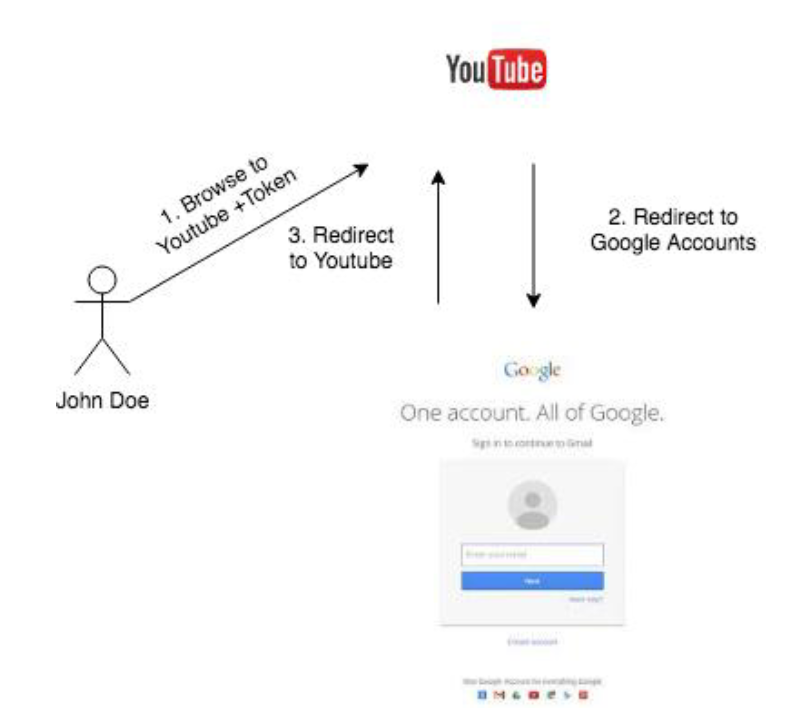
\includegraphics[width=0.6\textwidth]{images/8-1.png}
    \caption{Il service provider è anche l'identity provider.}
    \label{fig:8-1}
\end{figure}

\begin{figure}
    \centering
    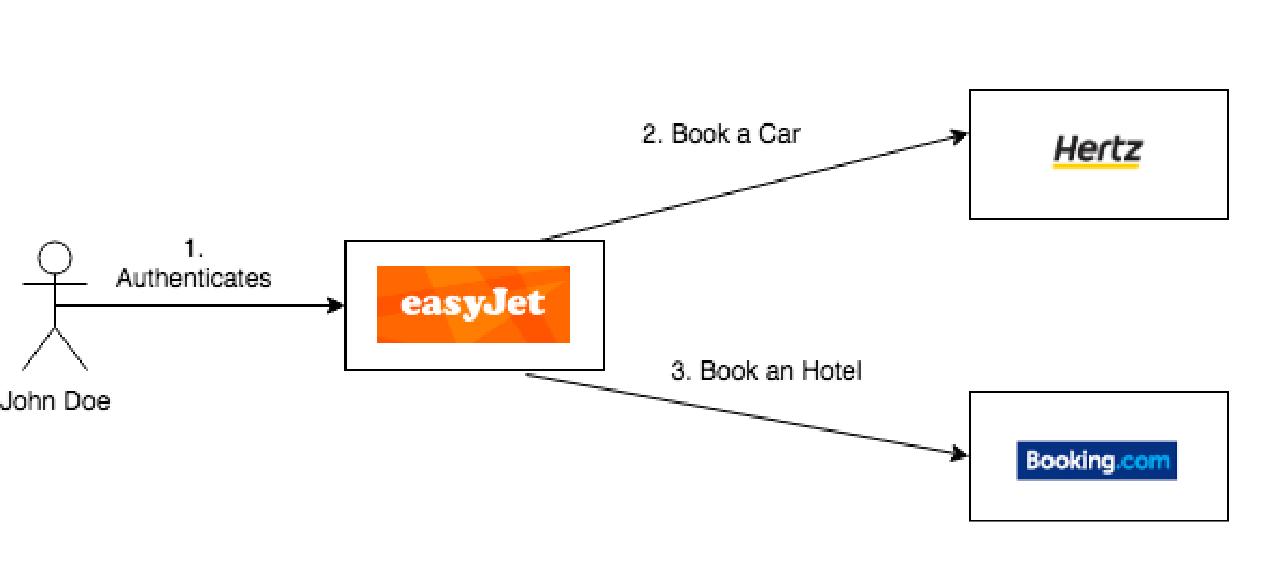
\includegraphics[width=0.6\textwidth]{images/8-2.png}
    \caption{Il service provider è diverso dall'identity provider.}
    \label{fig:8-2}
\end{figure}

\section{Identità federata}
L'identità federata sta alla base degli SSO cross domain. In questo caso diversi service provider decidono di fidarsi del processo di autenticazione effettuato da un altro service provider che fa parte della stessa federation. Qualsiasi entità della federazione può svolgere il ruolo di identity provider. 

\subsection{SPID}
Lo SPID è un esempio di sistema di identità federate in Italia. Con questo è possibile accedere ai servizi della PA e a quelli dei privati che hanno aderito alla federazione. 

\noindent I principali attori coinvolti nello SPID sono:
\begin{itemize}
    \item L'utente;
    \item L'Agenzia per l'Italia Digitale (AgID), che è l'entità che si occupa di accreditare tutti i fornitori di servizi e le entità che possono rilasciare lo SPID;
    \item L'Identity Provider, che è l'entità che rilascia l'identità digitale (es: Poste Italiane);
    \item Serivice provider;
    \item Attribute provider, che è responsabile di rilasciare gli attributi su cui viene poi rilasciata l'identità digitale. 
\end{itemize}

\noindent Lo SPID ha tre livelli di identità digitale, che corrisponde a tre diversi livelli di autenticazione sicura:
\begin{itemize}
    \item Il livello 1 lo SPID viene rappresentato da user e password;
    \item Il livello 2 richiede, oltre a quanto previsto per il livello 1,  anche un OTP che viene inviata tramite app o sms;
    \item Il livello 3 richiede, oltre a quanto previsto per i due livelli sopra, anche un dispositivo rilasciato dall'identity provider.
\end{itemize}

\noindent Con l'aumentare del livello di sicurezza aumentano anche i rischi se viene compromessa l'identità digitale.

\section{SAML}
Per implementare i sistemi di identità federate, è necessario un meccanismo standard per trasmettere info sul processo di autenticazione effettuato dall'identity provider e che deve essere validato dai service provider.

Il protocollo usato è SAML (Security Assertion Markup Language). Si tratta di un protocollo xml che consente agli identity provider e ai servide provider di scambiarsi attributi identificativi degli utenti e/o asserzioni per indicare che il processo di autenticazione ha avuto successo. 

Un tipico caso in cui il protocollo viene usato è quello della cross autentication (\ref{fig:8-3}).

\begin{figure}
    \centering
    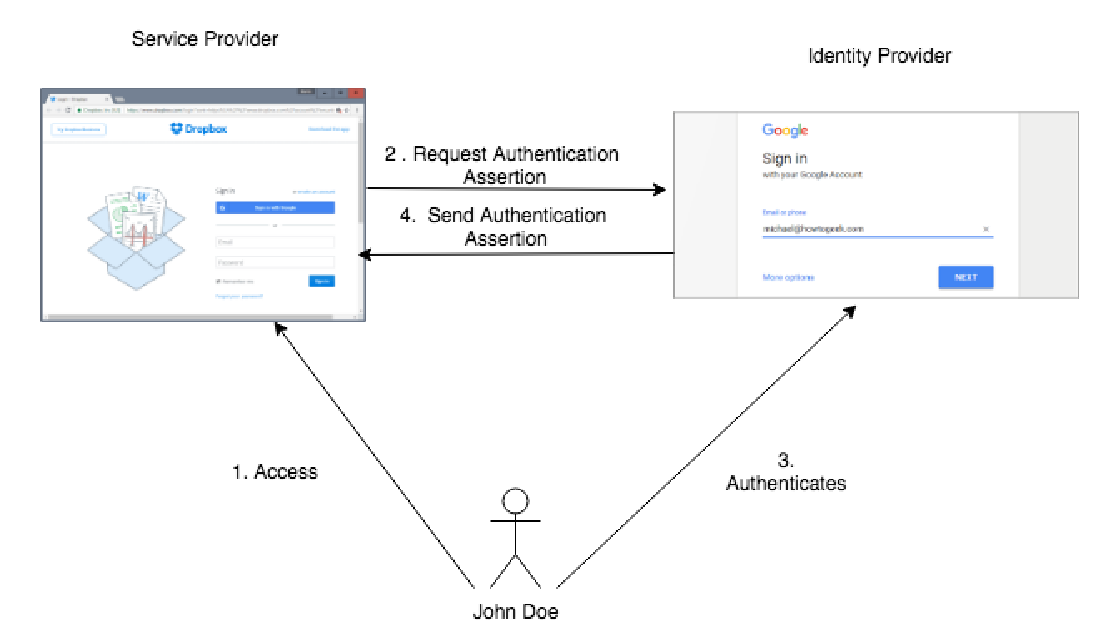
\includegraphics[width=0.6\textwidth]{images/8-3.png}
    \caption{La SAML Authenticatio Assertion di Goolge (prodotta in seguito alla request di Dropbox) specificherà quando è avvenuto il processo di autenticazione dell'utente, con quale modalità e per quanto tempo è valida l'autenticazione.}
    \label{fig:8-3}
\end{figure}



\subsection{Asserzioni SAML}

SAML permette di fare dichiarazioni su attributi posseduti da un soggetto (attribute assertion), sul processo di autenticazione effettuato dall'utente (authentication assertion) e sui permessi che sono garantiti all'utente sulle risorse fornite dal servizio online (authorization assertion). 

\noindent Tipicamente ogni asserzione contiene:
\begin{itemize}
    \item L'identity provider che ha rilasciato l'asserzione;
    \item Quando l'asserzione è stata generata;
    \item Un ID che consenta all'identity provider di distinguere l'asserzione dalle altre;
    \item Informazione relative al soggetto a cui è legata l'asserzione (nome e dominio a cui eventualmente appartiene);
    \item Condizione di validità (es: periodo di tempo, accesso solo a specifici servizi, ...).
\end{itemize}

\section{Shibboleth}
Altro protocollo che permette di implementare le identità federare. Si basa sullo standard di SAML. 
Viene usato principalmente per autenticare utenti che voglio accedere a risorse fornite da università o istituti di ricerca. Permette quindi di implementare il concetto di identità federate anche in ambito accademico. 

Un esempio di federazione accademica è la UK Access Management Federation, che raccoglie tutte le università inglesi. 

Prevede tipicamente tre identità: l'utente, il fornitore di servizi (università X) e l'identity provider (università Y). Quando l'utente prova ad accedere all'università Y, viene ridiretto al servizio WAYF (Where Are You Form), che gli consente di selezionare l'università X all'interno della federazione che fornisce le sue credenziali. A questo punto il servizio lo ridirige al servizio di autenticazione dell'università X selezionata che si occuperà di verificare la sua identità. Se la sessione di autenticazione ha acuto successo, l'università X genera un Handle che identifica la sessione di autenticazione (condiviso con Y). L'università Y, prima di concedere l'accesso ai suoi servizi online, rimanda l'Handle appena ricevuto e può richiedere attributi dell'utente per garantirgli l'accesso (potrebbe non accettare solo la prova dell'Handle). L'università X fornisce gli attributi aggiuntivi e l'università Y concede l'accesso all'utente.

\section{OpenID}

OpenID Connect (OIDC) è un protocollo di autenticazione aperto che profila ed estende OAuth 2.0 per aggiungere un livello di identità. OIDC consente ai client di confermare l'identità di un utente finale utilizzando l'autenticazione da parte di un Server di autorizzazione. L'implementazione di OIDC su OAuth 2.0 crea un unico framework che promette di proteggere API, applicazioni native mobili e applicazioni browser in un'unica architettura coesa.